\documentclass[12pt]{article}
\usepackage{graphicx}
\usepackage {color}
\usepackage{pdfpages}
\usepackage{float}
\usepackage{changebar}
\usepackage{enumitem,amssymb}
\renewcommand{\familydefault}{\sfdefault}
\usepackage[margin=1.2in]{geometry}
\usepackage{graphicx}
\usepackage{wrapfig}
\usepackage[super]{cite}
\usepackage{subcaption}
\usepackage[table]{xcolor}
\usepackage{amsmath}
\usepackage[sort, numbers]{natbib}
\usepackage{multirow}

%%%%%%%%%%%%Defining the margins %%%%%%%%%%%%%%%%%%%%%
\textheight 9.in
\textwidth 6.5in
\topmargin -.5in
\oddsidemargin 0in
\setlength{\parskip}{\smallskipamount}

%%%%%%%%%%%%%%Specific Commands %%%%%%%%%%%%%%%%%%
\newcommand{\eg}{{\em e.g.,}}
\newcommand{\ie}{{\em i.e.,}}
\newcommand{\etc}{{\em etc.,}}
\newcommand{\etal}{{\em et al.}}
\newcommand{\degrees}{{$^{\circ}$}}
\newcommand{\fig}[1]{\textbf{Figure #1}}

%%%%%%%%%%%%%%%%%%%%%%%%%%%% Setting to control figure placement
% These determine the rules used to place floating objects like figures 
% They are only guides, but read the manual to see the effect of each.
\renewcommand{\topfraction}{.9}
\renewcommand{\bottomfraction}{.9}
\renewcommand{\textfraction}{.1}
\renewcommand{\familydefault}{\sfdefault} %setting the san serif font

%%%%%%%%%%%%%%%%%%%%%%%% Line spacing
% Use the following command for ``double'' spacing
%\setlength{\baselineskip}{1.2\baselineskip}
% and this one for an acceptable NIH spacing of 6lpi based on 11pt
%\setlength{\baselineskip}{.9\baselineskip}
% The baselineskip does not appear to work when we include a maketitle
% command in the main file.  Something there must set the line spacing
% If we use this next command, then things seem to work.
\renewcommand{\baselinestretch}{.9}

\setcounter{secnumdepth}{0} %make no numbers but have a table of contents


\begin{document}

\title{Lab 1, Cow Heart, Lung, Kidney Dissection}
\author{Jake Bergquist, u6010393, Partner: Bram Hunt}
\maketitle

\section{Introduction}
\par{}
The purpose of this laboratory exercise was to dissect and explore the anatomy of a fresh bovine heart, lungs, and kidney. The physical exploration of these structures lead to a more in depth understanding of their function in the various systems in a living organism than can be attained from simple reading. Additionally real time dissections reveal features of anatomy not easily expressed in textbooks or descriptions such as texture, pliability, or the variations in structure apparent in individual specimens.

\par{}
An introduction of the basic function of these organs in their respective systems will facilitate a deeper understanding of the following discussion of the dissection. The common factor between these three organs (heart, lung, and kidney) is blood. Beginning first with the kidney, the basic function of this organ is to filter the blood of an animal to remove metabolic waste, balance the salt concentrations in the blood, and filter some toxins. The kidneys produce urine from these metabolic wastes and filtered toxins which is funneled to the bladder before excretion. Blood is brought into the kidneys where it is filtered across a semipermiable matrix called the glomerulus.\cite{Natsis2014a} This structure allows the plasma of the blood to pass into the nephrons while excluding large cells such as the blood cells. This fluid is then filtered through the nephrons via active and passive transport of water, ions, and metabolites such that waste remain in the nephrons the forming urea and water, nutrients, and ions can be reabsorbed back into the blood. The kidney is host to many nephrons which are organized into different sections called the renal cortex, medulla, renal pyramid, and renal columns. The collection of urine from these structures drains into a collecting duct called the minor calyx. As urine from several areas of the kidney collect in minor calyxes they form the major calyx which connects to the renal pelvis and ultimately the ureter. The ureter drains the urine to the bladder from whence it is excreted.\cite{Natsis2014a}
\par{}
Next we have the lungs which are responsible for the oygenation of the blood. Deoxygenated blood is fed into the blood where the capilary beds surround aviolar sacs. These sacs are an interface between the blood vessels and the air inspired into the lungs, where gas exchange can occur. Here deoxygenated blood absorbs oxygen from the aveoli while carbon dioxide is released so it can be expired from the lungs. The aviolar sacs are connected by a system of bronchi, which are hollow tubes that contain the air. These bronchi all merge together as branches of a tree merge to the trunk which in the case of the lung is the trachea. The trachea is connected to the mouth from where air is inhaled and exhaled.\cite{PMID:361341} Changes in the structure and organization of these airways in the lungs can result in numerous pathologies.\cite{Shaw2002}
\par{}
Finally we consider the heart. The purpose of the heart is to pump blood through the body via coordinated rhythmic muscular contraction. In the case of bovine, and mammalian hearts in general, the heart is divided into four chambers. Deoxygenated blood enters the heart from the body via the superior and inferior vena cava into the right atrium. The blood is pumped by the atria past the tricuspid valve into the right ventricle. From here the blood is pumped by the right ventricle through the pulminary valve into the pulminary artery and to the lungs. The blood is then oxygenated in the lungs and returned to the heart via the pulmonary veins into the left atrium. The blood is pumped by the left atrium past the bicuspid valve into the left ventricle. The left ventricle then pumps this oxygenated blood through the aortic valve to the body via the aorta. The two ventricles are separated by the cardiac septum. The heart itself is perfused by blood via the coronary arteries. Blood flows into these arteries via ostea found near the aortic valve on the aorta side of the valve. This blood is returned to the right atrium via the coronary sinus. The valves in the heart prevent blood from flowing in the wrong direction. In the case of the pulmonary and aortic valves they are held in place via the cordea tendinea, fibrous non conductive tissue that attaches the leaflets of the valves to the walls of the ventricles. This tissue is anchored to the ventricles of the heart via papillary muscles. The valves themselves are composed of thin, non conductive tissue that forms into a number of leaflets. These leaflets are roughly triangular in shape and when they come together they form a one way sealing valve that allows blood-flow in only one direction.\cite{Aurigemma2006}
\par{}
The pressures encountered in the heart vary, and as such the structure of the heart varies as well. In particular the ventricles are responsible for the primary muscular pumping of the blood. In the case of the right ventricle the blood that it pumps only needs to pass through the lungs and then reuturn to the heart. The left ventricle however must pump blood to the organs and structures of the entire rest of the body, including the heart itself. As such the pressures experience and generated by the left ventricle are much greater than those of the right. As such the structure of the left ventricle is very different to handle this different function. During this exploration of the cardiac dissection I will focus on the analysis of the left ventricle and how its structure relates to its function.


\section{Methods}
\subsection{Kidney Dissection}
\par{}
The kidney dissection began by clearing any non relevant fat tissue from the kidney and taking an initial size measure. The ureter was then identified and its diameter was measured. We then cut down the ureter to expose the renal pelvis and the beginning of the major calyx. Once the major calyx and minor calyxes were exposed diameter measures were taken. We then isolated one lobe of the kidney and split down the middle of the lobe in order to expose the renal pyramid and related structures.

\subsection{Lung Dissection}
\par{}
After separating the lungs from the heart we first inflated the lungs with compressed air. The lungs were inflated until the rate of expansion seemed to cease. We then noted the texture and pliability of the inflated vs the uninflated lungs. After the lungs had deflated we measured the diameter of the trachea. We then cut down the sides of the trachea until we reach a first generation brachial branch. The diameter was noted and we cut down on of these branches until we began to see second and third generation branches. The diameters of these branches as well as qualitative measures such as texture and pliability were measured.

\subsection{Cardiac Dissection}
\par{}
We began by carefuly dissecting the heart from the lungs. The heart and lungs we had to work with had a large amount of fatty and fibrotic tissue surrounding the lungs, as such it was difficult to fully separate the two without damaging the pulmonary veins. Once the heart was separated, we identified the left from right atria and ventricles and noted surface level vasculature. We also noted the location of two deep cuts in the heart inflicted by the butcher where the hearts were acquired.
\par{}
Dissection of the heart began with the superior and inferior vena cava. We measured the vein then cut from inferior to superior opening to expose the opening to the right atria. We then carfully cut the right atria open to expose the oracles as well as the tricuspid valve. We then moved to the pulmonary veins and cut then open to expose the left atria. The left atria was expose as the right. We then extended one of the butcher cuts through the septum by the right and left ventricle interface to separate the free wall of the right ventricle. This allowed for examination of the tricuspid valve, the right ventricular cavity, and the pulmonary valve. The pulminary valve and artery were split by the butcher cut, but were investigated as best as possible. Again on the anterior side the left ventricle free wall was separated from the septum. This allowed the investigation of the left ventricular cavity, the mitral valve, and the aortic valve. The aoric valve was split by the butcher cut. The aorta was then dissected from the pulmonary artery and investigated. We then cut down the pulimnary valve to identify the coronary ostia.


\section{Results}
\par{}
The anatomical measurement results are summarized in in Tables \ref{tab:heart},\ref{tab:kid},\ref{tab:lung}. Figure \ref{fig:H1} shows the heart at the beginning of dissection. There were large fatty deposits at the base of the heart which made identification of coronary vasculature difficult. The heart was also observed to have been stabbed twice by the butcher, once near the apex, and a second time through the right ventricle, septum, and part of the left ventricle. This cut both the pulmonary and aortic valves in half. Figure \ref{fig:H2} shows the atria after dissection. We see that the right atria is a deeper red in color while the left is whiter and was less pliable. A coronary sinus, a vein returning blood from the coronary vasculature to the right atrium was circled in figure \ref{fig:H2}.A. The Mitral and tricuspid valves can be seen through the atria in figure \ref{fig:H2}.C. In figure \ref{fig:H3} we see the ventricles cut away from the septum on the anterior side of the heart. While we quickly see the difference in wall thickness of the two ventricles, left being much thicker than the right, there are also a few other features. In \ref{fig:H3}.A we can see what appears to be a muscular moderator band, circled in green in front of the tricuspid valve. On the other side of the septum in figure \ref{fig:H3}.B we see what may be another moderator band, this time without muscle, in the left ventricle. Additionally we can clearly see the mitral valve cordea tendinea, as well as the cut made by the butcher to the right of the green circe in A and to the left of the green circle in B. We also note that the overall volume of the left venticle appears to be greater than that of the right. In figure \ref{fig:H4} we see a close up on all four valves of the heart. A and C give us our atrial ventricular valves, the tricuspid (A) and mitral (C) while B and D give the two ventricular-arterial valves, pulmonary (B) and aortic (D). Blood flows through these valves from A to B to C to D and so on. In A we can clearly see the three valves of the tricuspid held together, and held to the ventricular wall via the cordea tendinea. More cordea tendinea are highlighted in C for the mitral valve. B and D show the cup-like nature of the semiluminar valves. Unfortunately the butcher cut ran right through both of these valves. Finally in figure \ref{fig:H5} we see the aorta(A and C) and the pulmonary artery(B). We see that the aorta (C) is much thicker than the pulmonary artery(B). However the aorta is still rather flexible. We can see in (A) one of the two major branches we expect for a bovine aortic arch.
\par{}
In figure \ref{fig:L1} we see the results of the lung dissection, with the whole lungs in C, and the dissection of the trachea and bronchus in A and B. In C we can see that the right lung appears smaller than the left, and that there is an additional lobe on the right side. The bronchus of this additional node can be seen on the right in A, whereas the bronchi of the right and left major lobes are seen in A on the right and left respectively. In B we see a dissection down to several secondary bronchi, circled in green. The surfaces of the bronchi were smooth but rather rigid, like a hard rubber. The lung itself when inflated was soft and spongy. The lung inflated to roughly four times its deflated size.
\par{}
Figure \ref{fig:K1} shows the isolated kidney. Unlike human kidneys, the bovine kidney is lobular. The ureter seen in figure \ref{fig:K1} was very smooth and pliable. The lobes themselves felt very dense, similar to the density of the cardiac tissue. Figure \ref{fig:K2} details the anatomy of one of the lobes of the kidney. The major calyx which drains intot he pelvis is then connected to the ureter. Note the presence of repeating structures throughout the lobe.
\begin{table}[h]
	\centering{}
	\caption{Measurements from cardiac dissection.}
	\label{tab:heart}
\begin{tabular}{|r|r|r|r|}
	\hline
Structure & Measure & Value (mm) & Comment\\
\hline
\hline
\multirow{2}{*}{Whole Heart}
& Base Width & 230 & \\
& Apex Width & 180 & \\
\hline
\multirow{2}{*}{Vena Cava}
& inferior diameter & 30 & smooth, stretchy \\
& superior diameter & 40 & \\
\hline
Right Atrium & Oracle Depth & 40 & Smooth, spidery musculature\\
\hline
Right Ventricle & Free Wall Thickness & 20 & \\
\hline
Left Atrium & Oracle Depth & 20 & \\
\hline
Left Ventricle & Free Wall Thickness& 40&\\
\hline
Ventricular Septum & Thickness & 40 &\\
\hline
Mitral Valve & Depth/Length & 50 &\\
\hline
\multirow{2}{*}{Aorta}
&Main Diameter& 40&\\
&Branch Diameter & 20&\\
\hline
Aortic Valve&Depth/Length&30&\\
\hline
Left Main Coronary&Diameter& 4&\\
\hline
Right Main Coronary & Diameter& 4 & \\
\hline
Pulmonary Artery&Diameter&40&Cut by butcher\\
\hline
Pulmonary Valve & Depth/Length&45&Cut by butcher\\
\hline
Pulmonary Veins&Diameter&20&\\
\hline
Tricuspid Valve&Depth/Length&20&\\
\hline
\multirow{2}{*}{Cordea Tendinea}
&Average Length& 30&\\
&Average Width & 1 &\\
\hline

\end{tabular}
\end{table}
\begin{table}[H]
	\centering{}
	\caption{Measurements from lung dissection.}
	\label{tab:lung}
	\begin{tabular}{|r|r|r|r|}
		\hline
		Structure & Measure & Value (mm) & Comment\\
		\hline
		\hline
		\multirow{2}{*}{Trachea}
		&Diameter&30&hard, rubbery\\
		&Wall Thickness&3&\\
		\hline
		Left Main Bronchus&Diameter&25&smooth internal wall, hard\\
		\hline
		Right Main Bronchus&Diameter&25&\\
		\hline
		Second Generation Bronchus&Diameter&15&\\
		\hline
		
	\end{tabular}
\end{table}

\begin{table}[H]
\centering{}
\caption{Measurements from kidney dissection.}
\label{tab:kid}
\begin{tabular}{|r|r|r|r|}
	\hline
	Structure & Measure & Value (mm) & Comment\\
	\hline
	\hline
	\multirow{3}{*}{Whole Kidney}
	&Length&200&Lobed,smooth\\
	&Width&110&\\
	&Height&6&\\
	\hline
	Renal Cortex&Thickness&10&\\
	\hline
	Medulla&Thickness&20&\\

	\hline
	Renal Pyramids&height&30&\\	
	\hline
	Renal Columns&Length&25&\\
	\hline
	Minor Calyx&Diameter&5&\\
	\hline
	Major Calyz&Diameter&10&Smooth, stiff\\
	\hline
	Renal Pelvis&Dimensions&110x40x50&\\
	\hline
	Ureter&Diameter&1.75&Smooth,flexible\\
	\hline
	
\end{tabular}
\end{table}

\begin{figure}[H]

	\centering	
	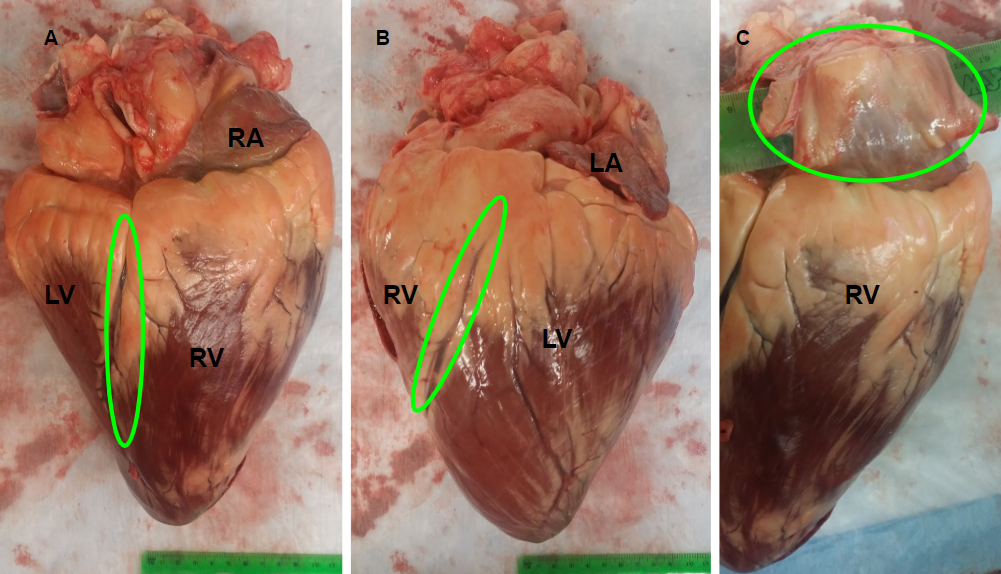
\includegraphics[width = 1\textwidth]{Figures/Heart1.png}
	\caption{ Initial heart view pre-dissection. (A) The heart viewed from the posterior. The posterior coronary is circled in green. (B) The heart viewed from the anterior. The left anterior descending coronary artery is circled in green. (C) The Superior and Inferior vena cava are shown and circled.}
	\label{fig:H1}
\end{figure}
\begin{figure}[H]
	
	\centering	
	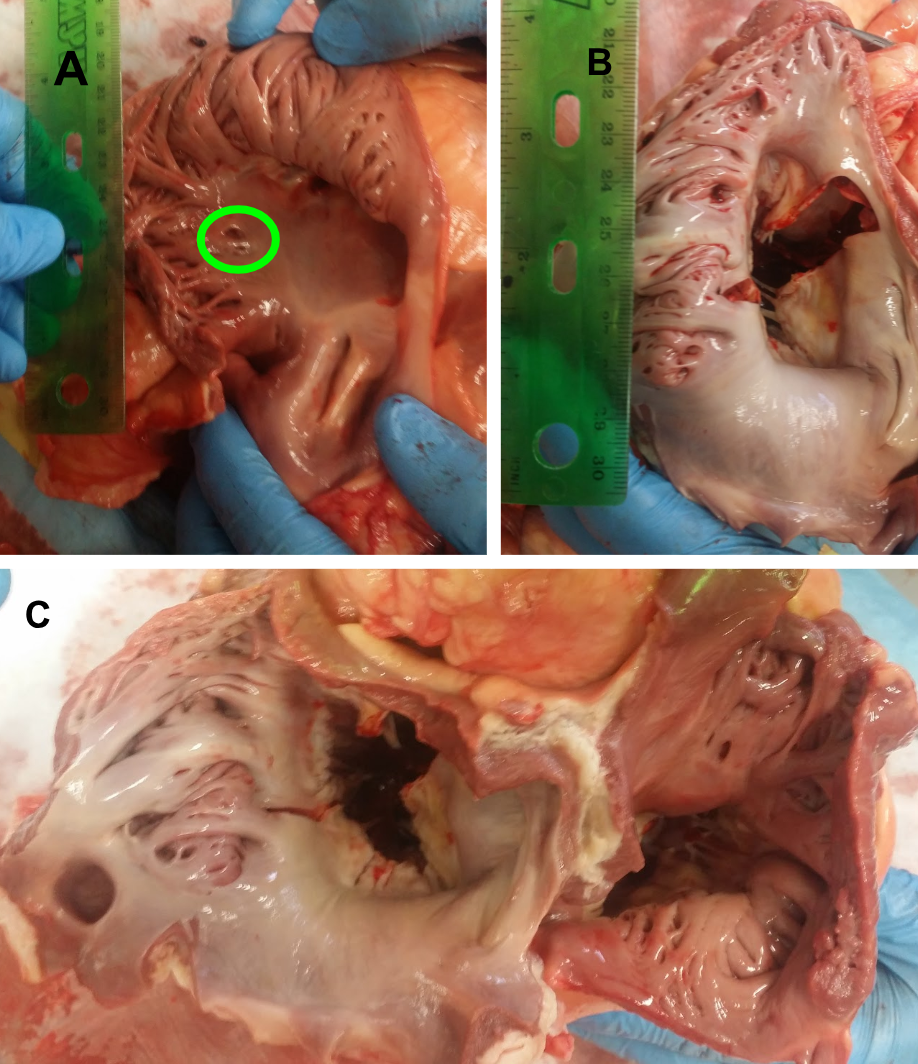
\includegraphics[width = 1\textwidth]{Figures/Heart2.png}
	\caption{Atrial dissection. (A) Right Atrium with coronary sinus circled in green, and (B) Left Atrium shown from a basal to anterior view. (C) Both atria can be seen with the right arium on the left and the left atrium on the right.}
	\label{fig:H2}
\end{figure}
\begin{figure}[H]
	
	\centering	
	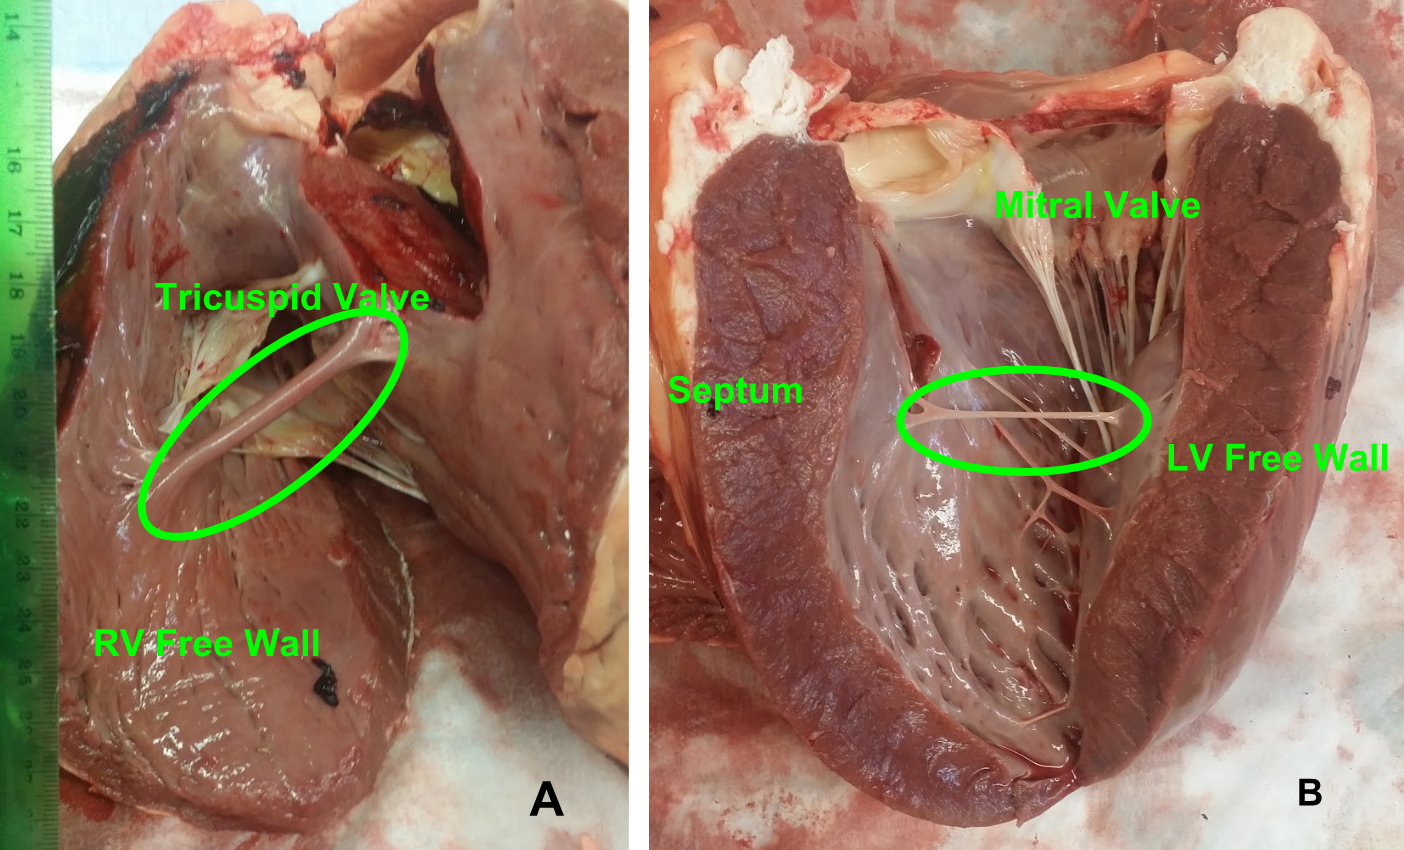
\includegraphics[width = 1\textwidth]{Figures/Heart3.png}
	\caption{ Ventricular dissection. (A) The right ventricle and (B) left ventricle are shown post dissection. The RV and LV free walls have been cut away from the septum from the anterior side. (A) The tricuspid Valve can be seen behind what appears to be a moderator band(circled in green). Additionally one of the butcher cuts can be seeen above the moderator band. (B) Another possible moderator band is circled in green. The Mitral valve can be seen at the top of the ventricle. }
	\label{fig:H3}
\end{figure}
\begin{figure}[H]
	
	\centering	
	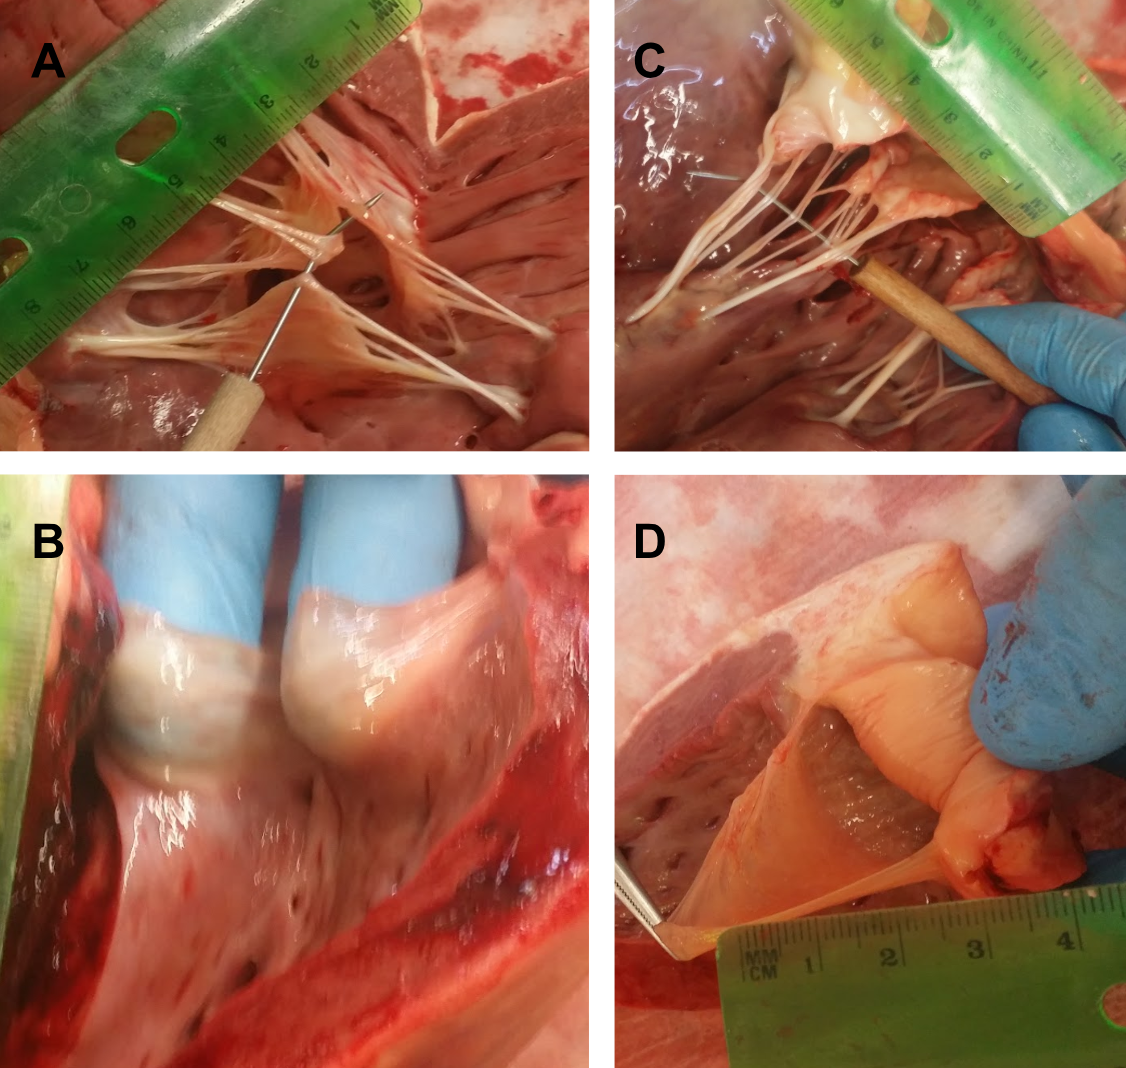
\includegraphics[width = 1\textwidth]{Figures/Heart4.png}
	\caption{ Valves. (A) The tricuspid valve and associated cordea tendinea, held together. (B) The pulminary semiluminar valve, with the butcher cut cutting through the valve. (C) The mitral valve and associated cordea tendinea. (D) The aortic valve, with the butcher cut cutting through the valve. }
	\label{fig:H4}
\end{figure}
\begin{figure}[H]
	
	\centering	
	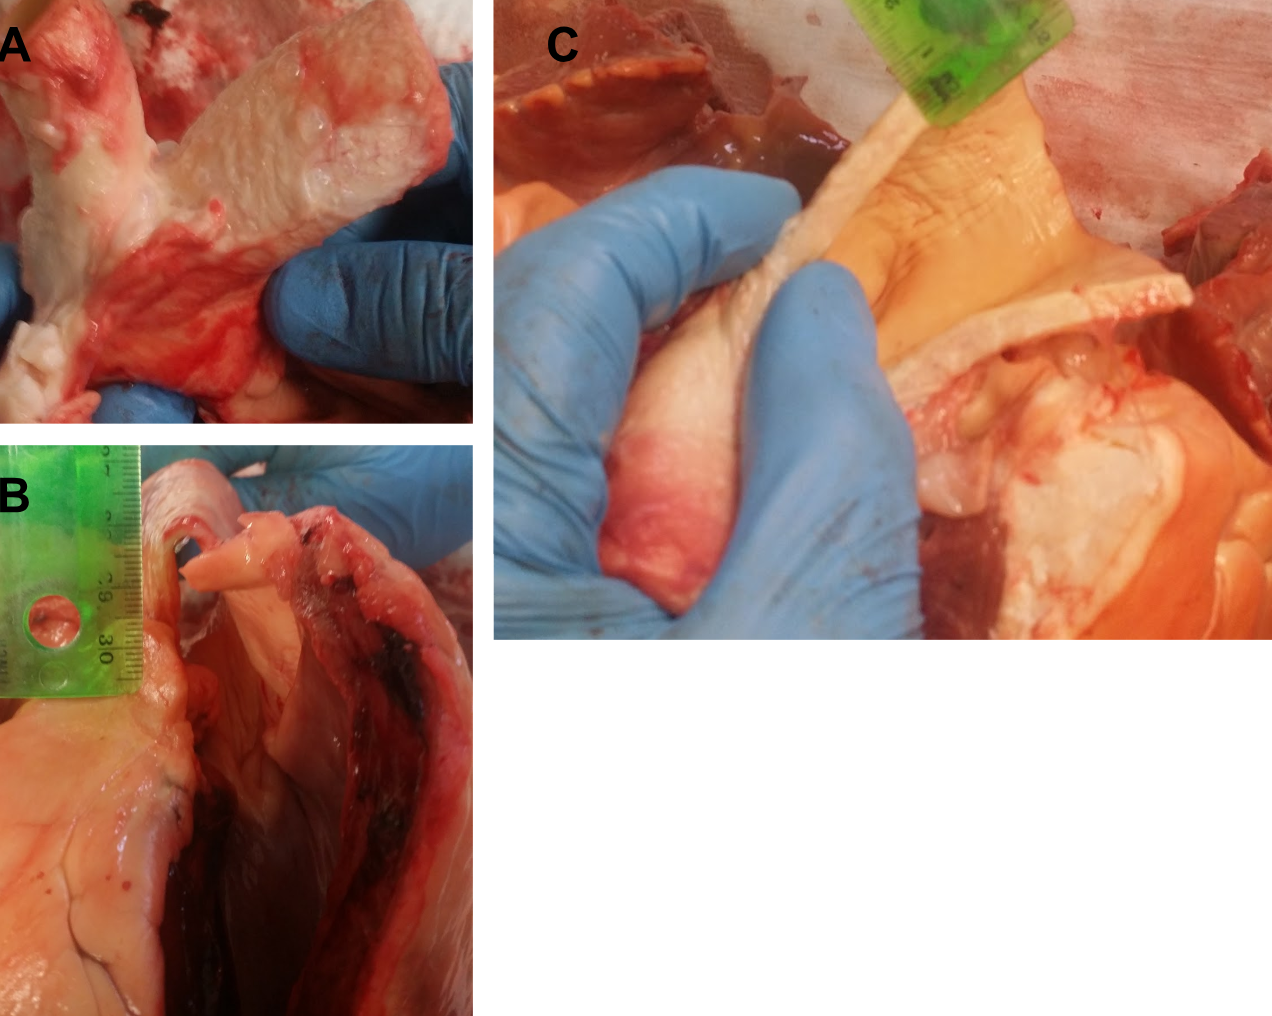
\includegraphics[width = 1\textwidth]{Figures/Heart5.png}
	\caption{The Aorta and Pulmonary Artery. (A) The aorta dissected from the pulmonary artery. (B) A view through the pulmonary artery. (C) The thickness of the Aorta was measured.}
	\label{fig:H5}
\end{figure}
\begin{figure}[H]
	
	\centering	
	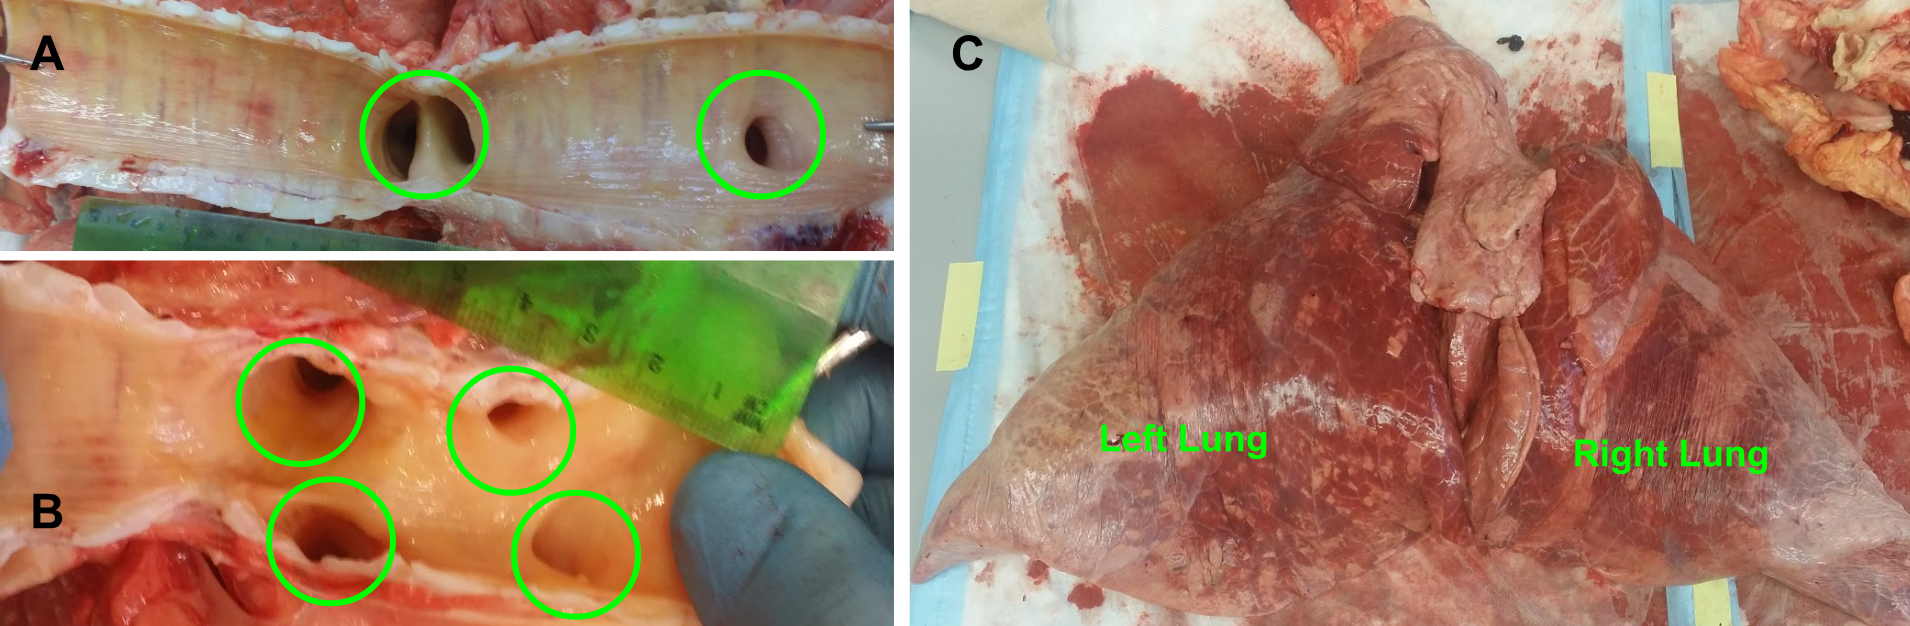
\includegraphics[width = 1\textwidth]{Figures/Lung1.png}
	\caption{The primary left and right brachia as well as an extra primary brachia are shown in A, circled in green. Second generation brachia are shown in B. The entire lungs are shown in C.}
	\label{fig:L1}
\end{figure}
\begin{figure}[H]
	
	\centering	
	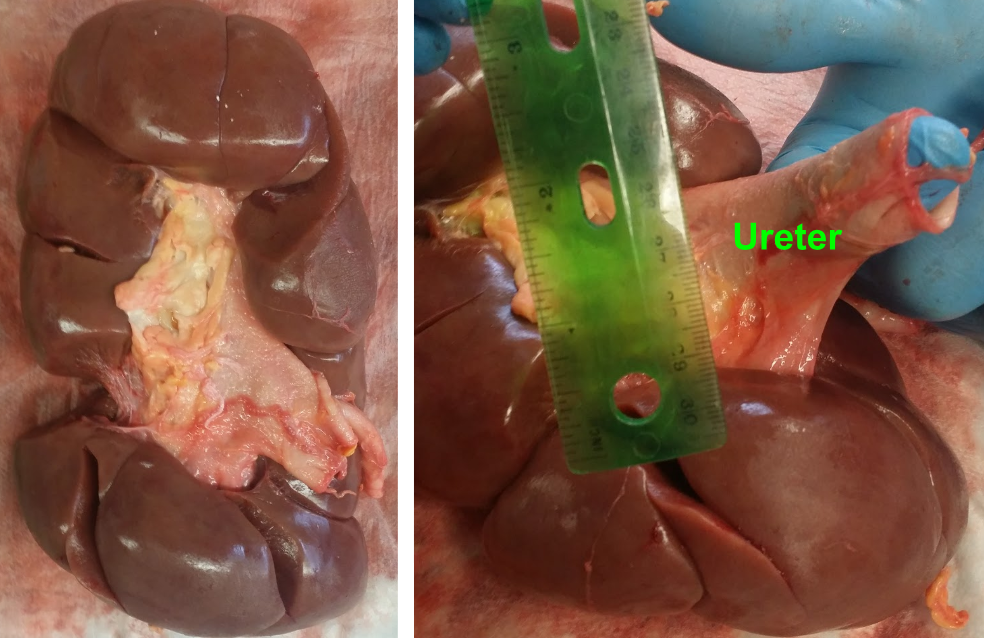
\includegraphics[width = 1\textwidth]{Figures/Kidney1.png}
	\caption{Kidney Overview. (A) The whole Kidney. (B) the Uereter.}
	\label{fig:K1}
\end{figure}
\begin{figure}[H]
	
	\centering	
	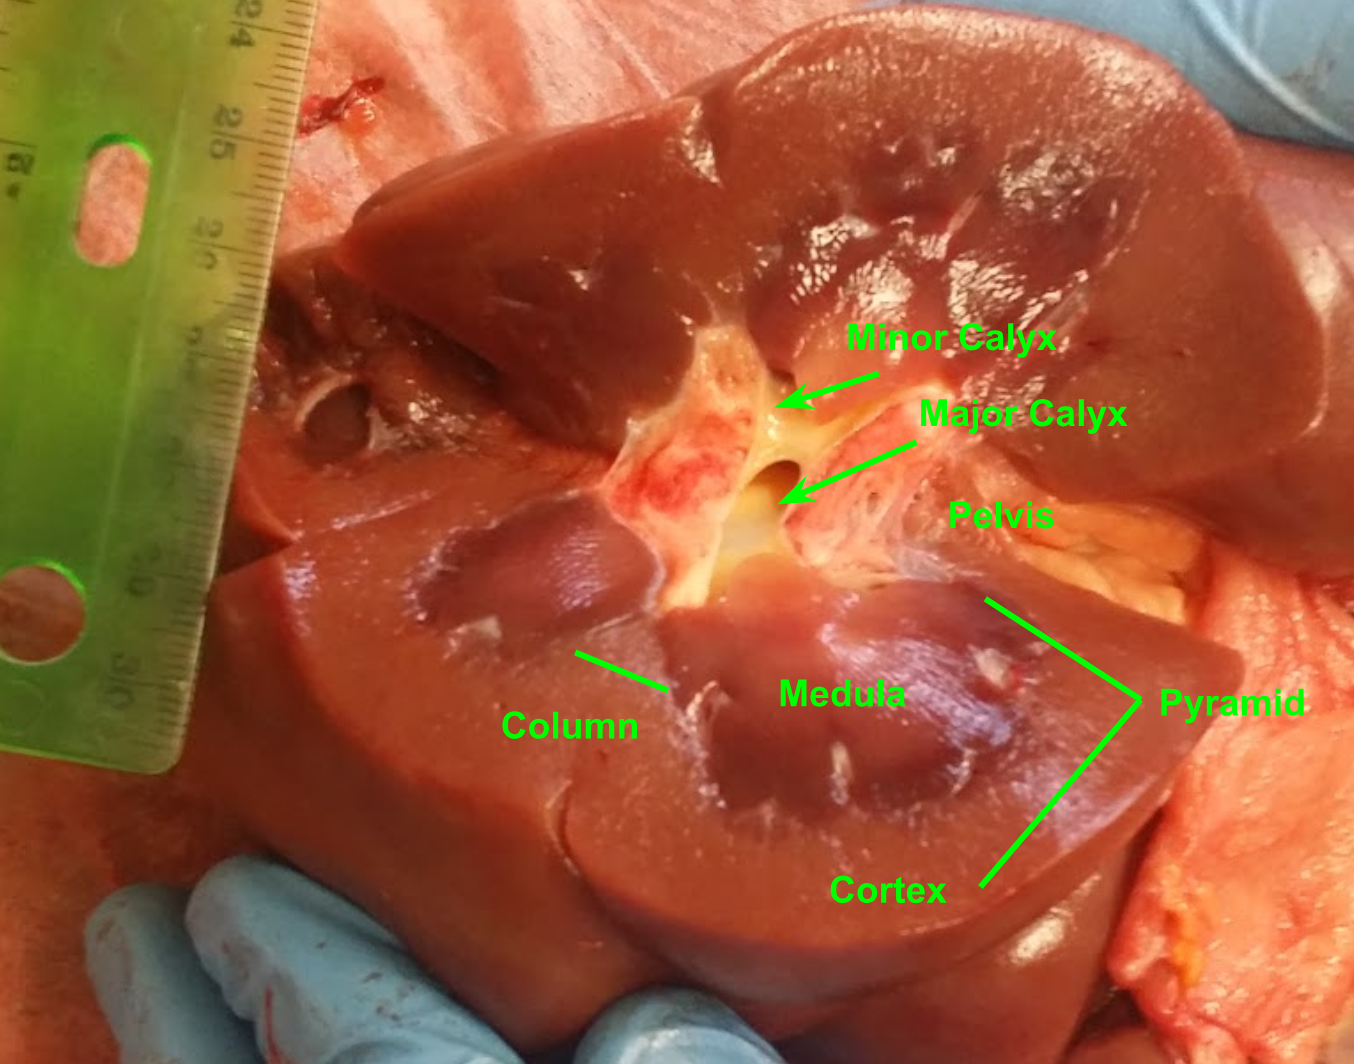
\includegraphics[width = 1\textwidth]{Figures/Kidney2.png}
	\caption{Kidney dissection. The structural elements of the kidney are identified in green.}
	\label{fig:K2}
\end{figure}

\section{Discussion}
\par{}
The goal of this laboratory exercise was to perform a general dissection of a bovine lungs, kidney, and heart in order to gain familiarity and an improved functional understanding of these organs. By performing this hands on dissection we gained an in depth understanding of the structures and accompanying functions of these organs in a way that allowed us to explore the properties we found interesting. Such an exploration results in an increase in understanding that cannot be attained from mere reading. The ability to manually manipulate and investigate the structures of these organs resulted in a functional understanding that bridges gaps in theoretical knowledge.
\par{}
During the dissection we investigated the lobular structure of the kidneys, which we found to be a repeating set of units where each lobe could be viewed as one unit. Within each lobe we were able to identify the functional structures of the kidneys such as the calyx, pelvis, and ureter, as well as the medulla, pyramid, columns, and cortex. During our investigation of the lungs we were able to follow the brachial tree down to the first generation branches to the left and right lung, as well as further to secondary and even tertiary branches. We were also able to explore the inflation and deflation of the lungs using compressed air. In the case of the cardiac dissection we were able to follow the flow of blood through the chambers and investigate each of the structures that make this process possible. All of these investigations led to a more functional knowledge and understanding of these organ systems. In particular I want to focus on the heart, with a particular emphasis on the left ventricle.
\par{}
The left ventricle is implicated in several cardiac disease states, and its thickness and function can be used as a metric of disease progress.\cite{Parfrey1996}\cite{Aurigemma2006} Thus a comprehensive understanding of its function can help understand its role in different disease processes. The left ventricle is responsible for pumping oxygenated blood to the entire body (excluding the lungs). This requires the generation of a large amount of pressure especially when considering that with each beat the left ventricle must send blood not only up to the head, and down to the feet, but also maintain enough pressure such that this blood makes it back to the heart. Given that the function is to generate such an enormous amount of force, it as a cconsequence is composed of a large amount of muscle. When compared to the right ventricle (Table \ref{tab:heart}, Figure \ref{fig:H3}) the right ventricle is over twice as thick. This added muscle allows the left ventricle to generate a significant amount of force on the blood. Additionally when we compare the right ventricle to the left further we can notice a few more interesting things. The shape of the left ventricle is like a cup, wherease the right ventricle is almost like an extra pocket sewn onto the left ventricle. If we consider that the septum is practically the same thickness as the left ventricle, this furthers the idea that the right ventricle is simply the right ventricular free wall sewn onto the left ventricle. Thus the majority of the motion, contraction, and overall activity is dominated by the left ventricle. The left ventricle wall is also significantly less compliant than the right. This is likely due to the increased thickness, but this can also serve a purpose. The left ventricle is exposed to very high pressures from its contraction. As such, if it were as compliant as the right ventricle it would not be able to maintain or even contract against this pressure. Thus the decreased pliability of the left ventricle contributes to its function of producing enough pressure to pump blood across the entire body. With this functional understanding one could estimate the response of the left ventricle to different disease states. An increase in blood pressure chronically would likely cause an increase in left ventricular thickness (or be caused by) as these higher pressures would require a thicker left ventricle to stand up to them. Additionally a disease that affects the function of the left ventricle, such as scarring from a myocardial infarction of the left ventricle, would likely result in decreased bloodflow globally to the body as the left ventricle is responsible for providing blood to the body.

\par{}
Structural changes in these organs can also have implications in various disease states, thus conducting such dissections as this is necessary to investigate such structural changes. By conducting gross anatomical dissections researchers can assess basic structure function relationships that then alow the development of hypothesis that drive further research. The understanding acquired from such dissections informs more tissue, cellular, and even biochemical studies.


%%%%%%%%%%%%%%%%%% Correct Bibliography Style

\bibliography{C:/Users/Jake/Documents/BibFiles/library}
\bibliographystyle{IEEEtran}


\end{document}








